% Copyright (c) 2010-2016 Casper Ti. Vector
% Public domain.
%
% 使用前请先仔细阅读 pkuthss 和 biblatex-caspervector 的文档,
% 特别是其中的 FAQ 部分和用红色强调的部分。
% 两者可在终端/命令提示符中用
%   texdoc pkuthss
%   texdoc biblatex-caspervector
% 调出。

% 采用了自定义的(包括大小写不同于原文件的)字体文件名,
% 并改动 ctex.cfg 等配置文件的用户请自行加入 nofonts 选项;
% 其它用户不用加入 nofonts 选项,加入之后反而会产生错误。
\documentclass[UTF8]{pkuthss}

% 使用 biblatex 排版参考文献,并规定其格式(详见 biblatex-caspervector 的文档)。
% 这里按照英文文献在前,中文文献在后排序(“sorting = ecnty”);
% 若需按照中文文献在前,英文文献在后排序,请设置“sorting = centy”;
% 若需按照引用顺序排序,请设置“sorting = none”。
% 若需在排序中实现更复杂的需求,请参考 biblatex-caspervector 的文档。
\usepackage[backend = biber, style = caspervector, utf8, sorting = none, giveninits = true, sortgiveninits = true]{biblatex}

% 按学校要求设定参考文献列表中的条目之内及之间的距离。
\setlength{\bibitemsep}{3bp}
% 对于 linespread 值的计算过程有兴趣的同学可以参考 pkuthss.cls。
\renewcommand*{\bibfont}{\zihao{5}\linespread{1.27}\selectfont}

% 设定文档的基本信息。
\pkuthssinfo{
	cthesisname = {硕士研究生学位论文}, ethesisname = {Master Thesis},
	ctitle = {Pandax-III中本底模拟及探测器分辨率研究}, etitle = {The Background Simulation and Detector Resolution Study in PandaX-III},
	cauthor = {乔颢},
	eauthor = {Hao Qiao},
	studentid = {1501210103},
	date = {2018年5月},
	school = {物理学院},
	cmajor = {粒子物理与原子核物理}, emajor = {Particle Physics and Nuclear Physics},
	direction = {高能方向},
	cmentor = {王思广}, ementor = {Prof.\ Siguang Wang},
	ckeywords = {其一,其二}, ekeywords = {First, Second}
}
% 载入参考文献数据库(注意不要省略“.bib”)。
\addbibresource{thesis.bib}

% 普通用户可删除此段,并相应地删除 chap/*.tex 中的
% “\pkuthssffaq % 中文测试文字。”一行。
\usepackage{color}
\def\pkuthssffaq{%
	% \emph{\textcolor{red}{pkuthss 文档模版最常见问题:}}

	% \texttt{\string\cite}、\texttt{\string\parencite} %
	% 和 \texttt{\string\supercite} 三个命令分别产生%
	% 未格式化的、带方括号的和上标且带方括号的引用标记:%
	% \cite{test-en},\parencite{test-zh}、\supercite{test-en, test-zh}。

	% 若要避免章末空白页,请在调用 pkuthss 文档类时加入 \texttt{openany} 选项。

	% 如果编译时不出参考文献,
	% 请参考 \texttt{texdoc pkuthss}“问题及其解决”一章
	% “上游宏包可能引起的问题”一节中关于 biber 的说明。
}

\begin{document}
	% 以下为正文之前的部分,默认不进行章节编号。
	\frontmatter
	% 此后到下一 \pagestyle 命令之前不排版页眉或页脚。
	\pagestyle{empty}
	% 自动生成封面。
	\maketitle
	% 版权声明。封面要求单面打印,故需新开右页。
	\cleardoublepage
	% Copyright (c) 2008-2009 solvethis
% Copyright (c) 2010-2017 Casper Ti. Vector
% All rights reserved.
%
% Redistribution and use in source and binary forms, with or without
% modification, are permitted provided that the following conditions are
% met:
%
% * Redistributions of source code must retain the above copyright notice,
%   this list of conditions and the following disclaimer.
% * Redistributions in binary form must reproduce the above copyright
%   notice, this list of conditions and the following disclaimer in the
%   documentation and/or other materials provided with the distribution.
% * Neither the name of Peking University nor the names of its contributors
%   may be used to endorse or promote products derived from this software
%   without specific prior written permission.
%
% THIS SOFTWARE IS PROVIDED BY THE COPYRIGHT HOLDERS AND CONTRIBUTORS "AS
% IS" AND ANY EXPRESS OR IMPLIED WARRANTIES, INCLUDING, BUT NOT LIMITED TO,
% THE IMPLIED WARRANTIES OF MERCHANTABILITY AND FITNESS FOR A PARTICULAR
% PURPOSE ARE DISCLAIMED. IN NO EVENT SHALL THE COPYRIGHT HOLDER OR
% CONTRIBUTORS BE LIABLE FOR ANY DIRECT, INDIRECT, INCIDENTAL, SPECIAL,
% EXEMPLARY, OR CONSEQUENTIAL DAMAGES (INCLUDING, BUT NOT LIMITED TO,
% PROCUREMENT OF SUBSTITUTE GOODS OR SERVICES; LOSS OF USE, DATA, OR
% PROFITS; OR BUSINESS INTERRUPTION) HOWEVER CAUSED AND ON ANY THEORY OF
% LIABILITY, WHETHER IN CONTRACT, STRICT LIABILITY, OR TORT (INCLUDING
% NEGLIGENCE OR OTHERWISE) ARISING IN ANY WAY OUT OF THE USE OF THIS
% SOFTWARE, EVEN IF ADVISED OF THE POSSIBILITY OF SUCH DAMAGE.

% 此处不用 \specialchap,因为学校要求目录不包括其自己及其之前的内容。
\chapter*{版权声明}
% 综合学校的书面要求及 Word 模版来看,版权声明页不需加页眉、页脚。
\thispagestyle{empty}

任何收存和保管本论文各种版本的单位和个人,
未经本论文作者同意,不得将本论文转借他人,
亦不得随意复制、抄录、拍照或以任何方式传播。
否则一旦引起有碍作者著作权之问题,将可能承担法律责任。

% 若需排版二维码,请将二维码图片重命名为“barcode”,
% 转为合适的图片格式,并放在当前目录下,然后去掉下面 2 行的注释。
%\vfill\noindent
%\includegraphics[height = 5em]{barcode}

% vim:ts=4:sw=4


	% 此后到下一 \pagestyle 命令之前正常排版页眉和页脚。
	\cleardoublepage
	\pagestyle{plain}
	% 重置页码计数器,用大写罗马数字排版此部分页码。
	\setcounter{page}{0}
	\pagenumbering{Roman}
	% 中英文摘要。
	% Copyright (c) 2014,2016 Casper Ti. Vector
% Public domain.

\begin{cabstract}
	\pkuthssffaq % 中文测试文字
	摘要
\end{cabstract}

\begin{eabstract}
	Test of the English abstract.
\end{eabstract}

% vim:ts=4:sw=4

	% 自动生成目录。
	\tableofcontents

	% 以下为正文部分,默认要进行章节编号。
	\mainmatter
	% 序言。
	\specialchap{序言}

随着物理学的发展,人们对于这个世界的理解也越来越深入。在粒子物理的相关研究中,组成世界的基本粒子一共有12种,分为6种夸克,3种带电轻子以及三种中微子。随着对于这十二种粒子的深入研究和理解,人们在量子场论的框架下构建了基于量子色动力学和弱点相互统一理论的标准模型(Standard Model, SM)。标准模型成功的解释了宇宙中物质的构成以及他们之间的相互作用,并被大量的实验所证明。尤其是2012年标准模型所预测的最后一种粒子——希格斯玻色子被发现,更是完美的符合了标准模型的预测。

在标准模型所描述的基本粒子中,中微子是其中性质十分的特殊,也是最神秘的一个。对中微子的研究最早可以追溯到1930年,奥地利物理学家泡利(Wolfgang Ernst Pauli)在一封解释$\beta$衰变问题的信中,提出了一种微小的电中性粒子以解释衰变中能谱连续的问题。这个假设被费米(Enrico Fermi)引入到了他的$\beta$衰变理论中\supercite{wilson1968fermi}。而后在
1956年,Clyde Cowan和Frederick Reines首次确认了电子中微子的存在\supercite{cowan1991detection},于是中微子揭开了它隐藏的面纱,被人们所渐渐了解。$\mu$中微子于1962年被Brookhaven国家实验室所发现\supercite{danby1962observation},而后知道2000年,最后一种中微子$\tau$中微子存在的直接证据才被费米实验室所找到\supercite{kodama2001observation}。

标准模型中中微子被认为是没有质量的,然而过往和正在进行的大量中微子实验,如超级神冈(Super-Kamiokande)\supercite{fukuda1998evidence},萨德伯里中微子观测站(SNO)\supercite{ahmad2002direct}等,都观测到了中微子震荡现象。对这些现象最为自然的解释就是中微子是有质量的,这也可能标志着标准模型之外的,未被探索的新物理。

中微子既然可能有质量,那么它质量的来源便是一个十分有趣的问题。如果假设中微子是狄拉克费米子(Dirac fermions),那么为了使中微子产生质量,中微子与希格斯场相互作用的耦合系数会比夸克等粒子小12个量级,这种模型解释起来会变得十分的困难。另一种假设是中微子是马约拉纳费米子(Majorana fermions),即中微子自身是自己的反粒子,这种模型相对而言更为自然自洽,但它也意味着标准模型中的轻子数守恒的推断将会被打破,这将会对理论物理带来巨大的改变。然而到现在为止,还没有足够的实验观测能够判断哪种模型更为正确。

在中微子到底是哪种费米字的相关研究中,有一类实验是在寻找被称作无中微子双Beta衰变(Neutrinoless double beta decay, NLDBD)\supercite{avignone2008double}的稀有事件。在标准模型中,有一些核素不能直接进行普通的Beta衰变,但是他们可以通过一个次级的弱相互作用来同时释放出两个电子(正电子)和两个反中微子(中微子),这种衰变模式被称作双Beta衰变(Double beta decay, DBD),这种衰变过程也已经被实验所观测到了。如果中微子是马约拉纳费米子,这就意味着中微子和反中微子完全一致,那么双Beta衰变中第一次释放出的反中微子(中微子)又可能作为中微子(反中微子)参与了第二次衰变,即直接衰变出两个电子(正电子)而不产生反中微子(中微子)。这种现象就被称作无中微子双Beta衰变(后称NLDBD)事件。

如果NLDBD事件被探测发现,那么不单单意味着轻子数不再守恒,中微子的质量也可以通过NLDBD事件的发生概率计算得到,如公式\ref{eq1}所示\supercite{avignone2008double}。其中$G^{0\nu}$是相空间因子,$M^{0\nu}$是核矩阵元素。如果能够测量得到NLDBD事件的半衰期,那么马约拉纳中微子质量$\langle m_{\beta\beta}\rangle$就可以计算得到,进而可以得到中微子绝对质量量级和中微子的质量顺序,使得人们对中微子能够获得进一步的认识。

\begin{equation}
    (T_{1/2}^{0\nu})^{-1}=G^{0\nu}|M^{0\nu}|^2\frac{\langle m_{\beta\beta}\rangle ^2}{m_e^2}
    \label{eq1}
\end{equation}

这些年来世界上很多实验组都在探测无中微子双Beta衰变,根据2015年11月美国核科学顾问局的报告\supercite{NLDBD_NSAC},现在正在进行的实验包括CUORE\supercite{Artusa:2014lgv},EXO-200\supercite{Albert:2014awa},GERDA
\supercite{Agostini:2016iid},KamLAND-Zen\supercite{KamLAND-Zen:2016pfg},
Majorana\supercite{Abgrall:2013rze},SNO+\supercite{Andringa:2015tza}等,最好的实验结果是KamLAND-Zen
给出的关于$^{136}$Xe的无中微子双Beta
衰变,其半衰期大于$1.07\times10^{26}$年。现在世界上的NLDBD
实验组普遍达成了共识,至少需要1吨级别的放射性同位素才有可能通过探测NLDBD
事件确定中微子的质量顺序。为了顺利的完成这一量级的实验,需要能够顺利的生产出吨级的同位素,同时需要极佳的探测器分辨率和极低的本底噪声,以及鉴别NLDBD
和本底的方法。

粒子和天气物理氙探测器第三期实验(Particle And Astrophysical Xenon Experiment III,以下简称PandaXIII)便是一个设计中的吨级的$^{136}$Xe无中微子双Beta衰变探测实验,它使用高压气氙时间漂移室(TPC)作为探测器,放置于锦屏地下实验室来屏蔽宇宙射线本底,并计划在两到三年内建立出第一个200kg级探测器。本文详细描述了PandaXIII实验设计和前期测试中模拟的相关工作,分为以下几个部分。第一章将会简单介绍整个项目,第二章描述了探测器模拟中本底模拟的相关工作,第三章介绍了如何使用卷积神经网络(Convolution Neural Network, CNN)来鉴别本底事件和信号,第四章给出了原型探测器测试标定过程中的模拟工作。上述工作是本文作者主要参与的,PandaXIII项目中探测器设计,电子学等其他相关工作的描述可以参见PandaXIII中期设计报告\supercite{cdr}。

% vim:ts=4:sw=4
	% 各章节。
	\chapter{PandaX-III项目介绍}
\label{chapter:intro}
%\pkuthssffaq % 中文测试文字。

正如上文所说,NLDBD 是一种极其稀有的事件,既有实验已经给出它的半衰期 $T^{0\nu}_{1/2}>1.07\times10^{26}$ 年。如果要由此计算出中微子质量顺序,那么至少需要 1 吨量级的衰变元素才有能达成该目标。所以 NLDBD 的相关实验需要解决以下难点:

\vspace{0.4cm}
\begin{enumerate}
    \item 顺利制造和生产出 1 吨以上有可能发生NLDBD事件的放射性元素。
    \item 建造出具有极佳的能量分辨率和位置分辨率的探测器,达到 NLDBD 事件探测的需求。
    \item 探测器本底噪声很低,在灵敏区域内的背景事件数目应小于 $10^{-4}$ \ckky。
    \item 寻找到高效区分 NLDBD 信号及背景事件的方法。
\end{enumerate}
\vspace{0.4cm}

本章节简单介绍了PandaX-III实验如何通过适当选择衰变元素及合理设计探测器结构等操作来解决上述困难,以够顺利达成探测 NLDBD 事件的实验目标。

\section{元素选择}

在诸多可以发生 NLDBD 事件的放射性元素中,\xeots 在自然界中同位素丰度较高,价格相对便宜,自身还可以作为气体探测器的工作气体,因此 PandaX-III 选取了它作为目标衰变元素。\xeots NLDBD 事件释放出的总能量为 $Q_{\beta\beta}=2458$keV,这个能量相对较高,能够避开部分低能背景辐射。但是在 $Q_{\beta\beta}$ 附近, $^{214}$Bi 和 $^{208}$Tl 两种元素的 $\gamma$ 衰变可能会对实验造成影响,其中 $^{214}$Bi 释放出的 $\gamma$ 射线能量为 2448keV,只比 $Q_{\beta\beta}$ 低10keV 左右。更为严重的是,这两种元素是 $^{238}$U 和 $^{232}$Th 衰变链的中间产物,他们广泛存在于生产生活中的各种材料中,因此降低探测器材料中 \utte 和 \thttt 对实验的影响是 PandaX-III 所面临的一个巨大挑战。

PandaX-III 使用了 10bar 的高压气氙作为探测气体,其中 \xeots 的丰度为 90\%。为了配合电子学读出系统并增强读出信号的质量,探测气体同时混合了 1\% 的 TMA(trimethylamine)。根据 NEXT 实验的相关研究,使用这种混合气体作为探测介质能够在 $Q_{\beta\beta}$ 处达到 3\% 的能量分辨率\supercite{azevedoh2015accurate}。

\section{探测器构造}
\label{section:detector}

PandaX-III 计划建造 5 个 200kg 级高压气氙时间漂移室(Time Projection Chamber, TPC)用于探测 NLDBD 事件,探测器结构如图\ref{fig:detector}左所示。高压气体TPC的相关技术在上个世纪 90 年代便已经成熟,它的能量分辨率远远优于液体TPC。如果使用直接采集电离电子的读取器件作为探测器读出系统,高压气体TPC的能量分辨率能够达到液体的10倍。高压气体TPC另外一个巨大的优势是它具有优秀的位置分辨本领,配合像素或者条状读出可以十分便捷的重建出事件的径迹。在寻找 NLDBD 的相关试验中,径迹信息可以用与高效的鉴别本底背景和 NLDBD 信号,从而可以极大的压低背景噪声,以满足实验极低本底的需求。本文第\ref{chapter:cnn}章着重介绍了使用深度卷积神经网络进行背景及信号鉴别的方法。

\begin{figure}[tbp]
    \centering
    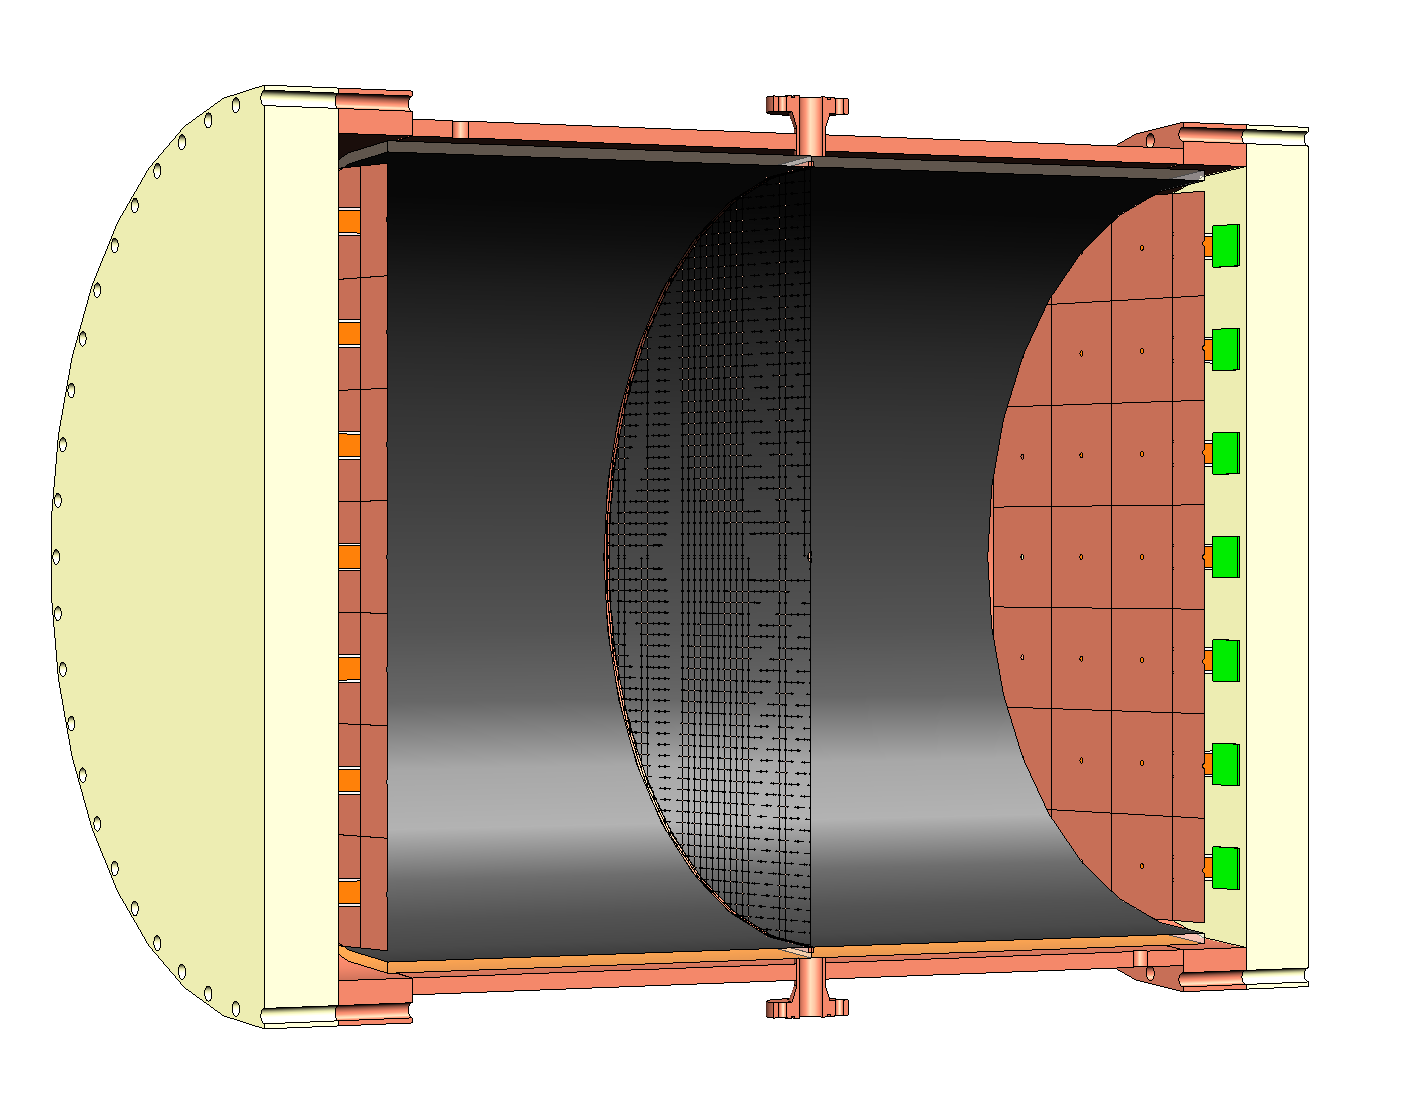
\includegraphics[width=0.4\columnwidth]{pic/fig1.png}
    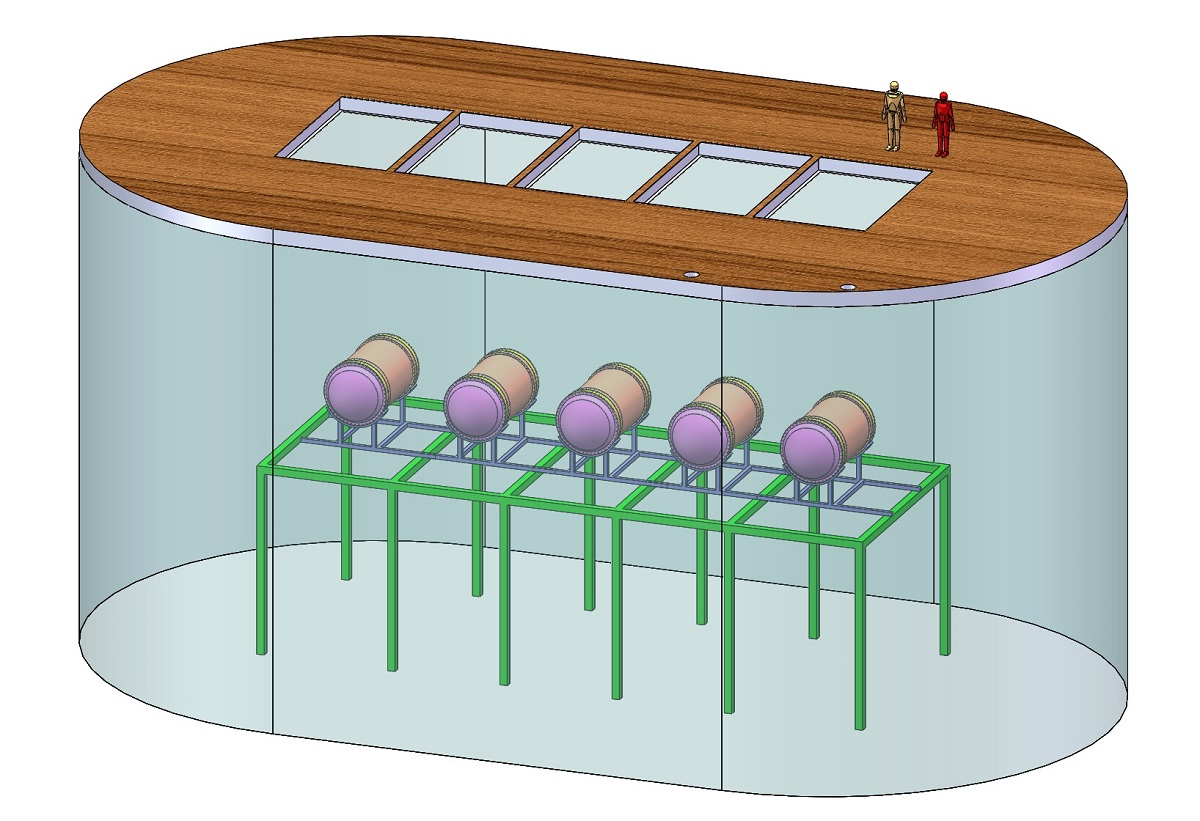
\includegraphics[width=0.4\columnwidth]{pic/fig2.jpg}
    \caption{左图:PandaX-III 实验中高压气氙 TPC 结构示意图。右图:放置在水池中的 5 个 TPC 所组成的 1 吨量级探测器示意图。\supercite{cdr}}
    \label{fig:detector}
\end{figure}
    
探测器主体是一个内高 2m,内直径 1.5m,使用高纯度无氧铜制作的柱形压力铜罐,总容积约为 3.5m$^3$。铜罐中心放置了圆形网状电极,内壁有等间隔的放置了 99 个圆形铜环,铜环之间以及铜环与内壁之间使用聚四氟乙烯(PTFE)隔离和支撑。这些铜环和极板共同组成一个场笼,为探测器提供了一个强度为 1kV/cm,延罐体轴心方向的漂移电场。铜罐壁厚度为 30mm,两端厚度为 150mm,放置于如\ref{fig:detector}右图所示的一个尺寸为 $27\times15\times13$m$^3$ 的水池中,利用超纯水来屏蔽周围环境的本底辐射。该水池建造在中国锦屏地下实验室中,利用实验室上方2500米厚的山岩屏蔽宇宙射线。对于探测器自身材料产生的本底辐射,PandaX-III 实验试图通过合理的探测器材料选择及结构设计来降低本底的数量。根据近年的研究,一些商业无氧铜材料中 \utte 和 \thttt 的含量可以低于0.1个 ppt(part per trillion)\supercite{abgrall2016majorana},是不锈钢材质的千分之一以上。本文在第\ref{chapter:background}章详细介绍了使用Geant4模拟分析得到的探测器本底事件组成。

\section{电子学以及读出}

为了提高探测器的能量分辨率,PandaX-III 实验使用了新型的被称作 Micromegas 的读出系统。它通过直接收集电离后的漂移电子来产生信号,结构简单,能量分辨率高,也容易控制自身材料带来污染。根据现有的针对 Microbulk Micromeags(一种 Micromegas,后称 MM)读出系统的详细研究,在 $Q_{\beta\beta}$ 附近使用它作为 10Bar Xe+TMA TCP 的读出,探测能够达到 3\% 的能量分辨率。PandaX-III 实验前期会直接向 CERN(European Organization for Nuclear Research,欧洲核子研究中心)订购 Microbulk Micromegas 成品,在实验的中后期则会尝试对读出系统做进一步的改进和优化以达到更佳的能量分辨率\supercite{cdr}。

在配合读出系统的电子学部件中,电子电气元器件很难做到放射性洁净,而且PCB板中的部分电路可能会游离出电子,为实验带来较大的背景污染。因此在探测器设计中,电子学部分被放置在铜罐两端外,使用 150mm 厚度的铜体来屏蔽它产生的背景辐射。同时为了能够重建出事件的径迹,读出系统需要做到像素读出或者是条状读出,为此所引入的大量通道数目也为电子学设计提出了挑战。PandaX-III 中期设计报告\supercite{cdr} 中详细描述了电子学以及数据获取系统的设计过程。

\section{PandaX-III实验设计总结及模拟工作}

为了探测寻找到NLDBD这样一极其稀有的事件,PandaX-III 实验在各个方面上都做了细致的考虑和设计,总结如下:

\vspace{0.4cm}

\begin{itemize}
    \item 提高探测器的灵敏度。
    \begin{itemize}
        \item 使用 10bar Xe+TMA 气体构建的 TPC 探测器。
        \item 使用新型 Microbulk MicroMegas 读出系统直接捕获漂移电子。
    \end{itemize}
    \item 减少本底辐射。
    \begin{itemize}
        \item 使用低本底材料构建探测器。
        \item 将探测器放置于中国锦屏地下实验室中的高纯水水池中,以此屏蔽宇宙射线以及环境中的本底辐射。
        \item 通过合理的探测器结构设计减少一些由材料带来的本底辐射。
    \end{itemize}
    \item 寻找合适的算法高效鉴别NLDBD信号和背景事件,以提高探测器的探测效率。
\end{itemize}

\vspace{0.4cm}

在这些设计的过程中,模拟工作发挥了相当的重要作用,它为整个实验提供了的数据支持。通过模拟我们可以测试不同设计时探测器灵敏度的差异,可以计算使用不同材料时本地辐射的变化,从而利用这些数据来指导探测器的设计。模拟工作也有助与读出系统及电子学的优化,为探测器标定的设计提供参考。在 PandaX-III 实验前期建造原型探测器验证的相关工作中,模拟数据可以验证测试结果,解释未知问题。可以说模拟工作是PandaX-III实验中相当重要的一环,本文在后续章节中详细介绍了这些模拟工作。

% vim:ts=4:sw=4

	% 结论。
	% Copyright (c) 2014,2016 Casper Ti. Vector
% Public domain.

\specialchap{结论}
\pkuthssffaq % 中文测试文字。

PandaXIII 实验是一个使用高压气氙时间漂移室,探寻 \xeots 无中微子双 Beta 衰变 (NLDBD) 事件的实验。NLDBD 极其稀有少见,因而探测它需要极低的探测器本底以及较高的探测器效率。

通过对探测器进行蒙特卡罗模拟,本文得到了不同探测器组件对于本底的贡献。绝大部分的本底信号来自于 MicroMegas 读出板以及固定探测器铜罐的螺钉,而其他探测器组件以及环境对本底的贡献要小得多。最终计算得到整个实验的本底水平约为 $3.08\times 10^{-3}$count\/(keV$\cdot$kg$\cdot$y),即对于 PandaXIII 前期计划的 200kg 量级探测器而言,每年的本底计数约为 78 个。

这一本底水平还是高于实验的预期,因而本文测试了使用深度卷积神经网络进行事件鉴别,以此在不影响探测效率的情况下压低背景。本文使用蒙特卡洛产生的 $\gamma$ 本底以及 NLDBD 信号的训练了 Resnet50 网络,测试显示它可以在压低本地信号 175 倍的同时达到 47.5\% 的信号效率,比 PandaXIII 中期设计报告中的目标提升了 64\%。结合探测器背景模拟的数据后,PandaXIII 实验所设计的 1 吨量级探测器在经过 3 年的取数后,可以将 \xeots NLDBD 事件半衰期下限提升至 $1.6\times10^{27}$ 年。

在 PandaXIII 模拟以及重建工作外,作者也探究了如何使用 GPU 加速 Roofit 拟合过程。因为中微子本征能谱跨度较大,所以在描述探测到的能谱时探测器分辨率本身随能量连续变化的情况应该被考虑。此时传统使用 CPU 进行拟合分析的方法过于缓慢,无法保障时间要求。本文研究了利用 GPU 来加速数值积分过程,测试显示:当计算节点数目较多,如 $10^{6}$ 个节点时,利用文中的方法 GPU(型号:K80)相较于 CPU(型号:E2603v3)能够带来最多 218 倍的速度提升。


% vim:ts=4:sw=4


	% 正文中的附录部分。
	\appendix
	% 排版参考文献列表。bibintoc 选项使“参考文献”出现在目录中;
	% 如果同时要使参考文献列表参与章节编号,可将“bibintoc”改为“bibnumbered”。
	\printbibliography[heading = bibintoc]
	% 各附录。
	% Copyright (c) 2014,2016 Casper Ti. Vector
% Public domain.

\chapter{PandaXIII其他的TPC设计中的模拟工作}
%\pkuthssffaq % 中文测试文字。

PandaXIII中除了设计了如节\ref{section:detector}中所描述探测器结构外,还设计了其他的探测器结构加以测试。在原设计中铜罐自身即为压力容器,所以需要使用不锈钢钉进行铆合,带来了较大的本底,同时铜相对较软,作为压力容器可能会带来一定的风险,所以实验就设计了使用强度更强的,质量更轻的钛罐作为压力容器,内部衬铜完全作为屏蔽结构,以期待来带更好的屏蔽效果。

\begin{table*}[hbt]
    \begin{center}
        \begin{tabular*}{0.75\textwidth}{@{\extracolsep{\fill}}ccccc}
        \hline
        \hline
        \textbf{组件}   &   \textbf{参数}   &   \textbf{值} &   \textbf{材料} & \textbf{质量} \\ \hline
        \multirow{3}{*}{钛罐} 
            &   内径&   85\,cm&     \multirow{3}{*}{钛} &   \multirow{3}{*}{855 kg} \\
            &   高度&   210\,cm&    &   \\   
            &   壁厚&   1.5\,cm&    &   \\\hline
        \multirow{2}{*}{钛盖} 
            & 直径 & 91.5\,cm & \multirow{2}{*}{钛} & \multirow{2}{*}{1758 kg} \\
            & 厚度 & 7.5\,cm &  &    \\\hline
        \multirow{2}{*}{铜衬底} 
            & 内径 & 80\,cm & \multirow{2}{*}{铜} & \multirow{2}{*}{6678 kg} \\
            & 内高 & 200\,cm &  &    \\
            & 厚度 & 5\,cm &  & \\\hline
        \multirow{2}{*}{螺钉} 
            & 直径 & 1.4\,cm & \multirow{2}{*}{不锈钢} & \multirow{2}{*}{94.6 kg} \\
            & 高度 & 20\,cm &  &    \\
        \hline
        \hline
        \end{tabular*}
        \caption{钛罐组成部件的几何参数,材料以及质量表。\supercite{cdr}}
        \label{tab:ti_structure}
    \end{center}
\end{table*}

探测器设计尺寸表\ref{tab:ti_structure}所示。虽然钛罐子自身质量很轻,但是因为工艺原因该材料放射性清洁程度极差,在模拟中我们认为\utte的活度为90\uBqkg,而\thttt的活度为
230\uBqkg。不考虑探测器响应的模拟结果如表所示\ref{tab:ti_bck}所示。可以看出虽然来自于螺钉的本底事件被压低了一些,但是钛罐自身产生的本地辐射太强,远远高于铜罐的设计。

\begin{table*}[hbt]
    \centering
    \begin{tabular*}{\textwidth}{@{\extracolsep{\fill}}lcccc}
      \hline
      \hline
      \textbf{组件}&\textbf{元素}&\textbf{放射性活度}&\textbf{\multirow{2}{5em}{\centering 本底计数\\计数/年}}&\textbf{ \multirow{2}{8em}{\centering BI\\$10^{-5}c\/(keV\cdot kg\cdot y$)}}\\\\
      \hline
        \multirow{2}{8em}{钛罐罐体} 
            & $^{238}$U  &  90 $\mu$Bq/kg & 10.7 &  43  \\
            & $^{232}$Th & 230  $\mu$Bq/kg & 233.4 & 892 \\ \hline
        \multirow{2}{8em}{钛罐盖子}
            & $^{238}$U  & 90 $\mu$Bq/kg  & 5.8 &  23.2 \\
            & $^{232}$Th & 220 $\mu$Bq/kg & 132.7 & 530  \\
            \hline
         \multirow{2}{8em}{不锈钢螺钉}              
            & $^{238}$U   &  0.5 mBq/kg & 1.4 & 5.6  \\
            & $^{232}$Th  & 0.32 mBq/kg & 6.5 &  26.7 \\ \hline
        \multirow{2}{8em}{铜衬底}            
            & $^{238}$U  & 0.75 $\mu$Bq/kg  & 2.74 & 11 \\
            & $^{232}$Th & 0.2 $\mu$Bq/kg & 7.2& 29 \\
             \hline
      \hline
      \hline
    \end{tabular*}
    \caption{钛罐设计中罐体以及螺钉对本底贡献表。}
    \label{tab:ti_bck}
  \end{table*}


  在发现5cm厚的铜衬底不足以屏蔽来自钛罐的本底时,我们继续测试了使用更厚的10cm铜衬底的效果,此时探测器的结构如表\ref{tab:ti_structure_big},不考虑探测器响应的本底结果如表\ref{tab:ti_bck_big}所示。此时本地强度依然是纯铜罐设计的5倍左右,完全不能够被接受,因此在目前的设计中还是直接使用铜罐作为压力容器。如果我们能够找到更为洁净的钛以及不锈钢材料那么还是有可能更换设计的。

  \begin{table*}[hbt]
    \begin{center}
        \begin{tabular*}{0.75\textwidth}{@{\extracolsep{\fill}}ccccc}
        \hline
        \hline
        \textbf{组件}   &   \textbf{参数}   &   \textbf{值} &   \textbf{材料} & \textbf{质量} \\ \hline
        \multirow{3}{*}{钛罐} 
            &   内径&   90\,cm&     \multirow{3}{*}{钛} &   \multirow{3}{*}{1957 kg} \\
            &   高度&   220\,cm&    &   \\   
            &   壁厚&   1.5\,cm&    &   \\\hline
        \multirow{2}{*}{钛盖} 
            & 直径 & 96.5\,cm & \multirow{2}{*}{钛} & \multirow{2}{*}{1758 kg} \\
            & 厚度 & 7.5\,cm &  &    \\\hline
        \multirow{2}{*}{铜衬底} 
            & 内径 & 80\,cm & \multirow{2}{*}{铜} & \multirow{2}{*}{14130 kg} \\
            & 内高 & 200\,cm &  &    \\
            & 厚度 & 10\,cm &  & \\\hline
        \multirow{2}{*}{螺钉} 
            & 直径 & 1.4\,cm & \multirow{2}{*}{不锈钢} & \multirow{2}{*}{94.6 kg} \\
            & 高度 & 20\,cm &  &    \\
        \hline
        \hline
        \end{tabular*}
        \caption{加厚钛罐组成部件的几何参数,材料以及质量表。\supercite{cdr}}
        \label{tab:ti_structure_big}
    \end{center}
\end{table*}

  \begin{table*}[hbt]
    \centering
    \begin{tabular*}{\textwidth}{@{\extracolsep{\fill}}lcccc}
      \hline
      \hline
      \textbf{组件}&\textbf{元素}&\textbf{放射性活度}&\textbf{\multirow{2}{5em}{\centering 本底计数\\计数/年}}&\textbf{ \multirow{2}{8em}{\centering BI\\$10^{-5}c\/(keV\cdot kg\cdot y$)}}\\\\
      \hline
        \multirow{2}{8em}{钛罐罐体} 
            & $^{238}$U  &  90 $\mu$Bq/kg & 1.6 &  6.4  \\
            & $^{232}$Th & 230  $\mu$Bq/kg & 45.0 & 180 \\ \hline
        \multirow{2}{8em}{钛罐盖子}
            & $^{238}$U  & 90 $\mu$Bq/kg  & 2.2 &  8.7 \\
            & $^{232}$Th & 220 $\mu$Bq/kg & 28.1 & 112  \\
            \hline
         \multirow{2}{8em}{不锈钢螺钉}              
            & $^{238}$U   &  0.5 mBq/kg & <0.1 & <0.6  \\
            & $^{232}$Th  & 0.32 mBq/kg & 0.97 &  3.9 \\ \hline
        \multirow{2}{8em}{铜衬底}            
            & $^{238}$U  & 0.75 $\mu$Bq/kg  & 3.1 & 12 \\
            & $^{232}$Th & 0.2 $\mu$Bq/kg & 8.1& 32 \\
             \hline
      \hline
      \hline
    \end{tabular*}
    \caption{加厚钛罐设计中罐体以及螺钉对本底贡献表。}
    \label{tab:ti_bck_big}
  \end{table*}

% vim:ts=4:sw=4


	% 以下为正文之后的部分,默认不进行章节编号。
	\backmatter
	% 致谢。
	% Copyright (c) 2014,2016 Casper Ti. Vector
% Public domain.

\chapter{致谢}
%\pkuthssffaq % 中文测试文字。

时光飞逝,转瞬间我已经在燕园度过了难忘的 7 个春秋,也将完成我的学生生涯,真正的踏入社会中。于此时此地回首过往,在这接近于人生的十分之一的时间里,我从一个茫然无知的高中生逐渐成长,学习了许多也收获了许多,最终留下了无数宝贵的回忆。

在这段快乐学习生活的时光里,我要感谢陪我一起走来的老师,同学,朋友和家人们。首先我要感谢的便是我的导师王思广老师,感谢他在学习和科研上对我的的指导,以及在生活上对我的的关心和照顾。我也要感谢谌勋老师在 PandaXIII 研究中带领我一路走来。这两位老师严谨的治学态度,渊博的学识以及平易近人的人格魅力对我影响深远,是我一生都值得学习的榜样!

其次我要感谢我的同学和舍友们,感谢你们在生活中对我的关照。在这三年愉快的记忆中到处都是你们的身影,谢谢你们的陪伴。我也要感谢父母对我的养育以及毫无保留的支持,感谢你们在我身后的默默付出。你们的健康和幸福是我今生最大的愿望。

最后我也感谢学校对我的培养,祝您百廿生日快乐。
% vim:ts=4:sw=4

\chapter{科研情况统计}

\begin{enumerate}
\item 论文 "Signal-background discrimination with convolutional neural networks in the PandaX-III experiment using MC simulation" 将以第一作者发表于 <SCIENCE CHINA Physics, Mechanics \& Astronomy>, 已接受。
\item 论文 《利用GPU加速信号形状与探测器分辨率随能量变化的卷积》将以第一作者发表于《核技术》, 已接受。
\item 论文 "PandaX-III: Searching for Neutrinoless Double Beta Decay with High Pressure 136Xe Gas Time Projection Chambers" 合作组文章已发表于 <Science China Physics, Mechanics \& Astronomy>, 本人主要参与了其中背景模拟的相关工作。
\item 论文 "Simulation Study of the Performance of New Micro Pattern Gaseous Detectors" 以第四作者发表于 <Radiation Detection Technology and Methods> 。
\end{enumerate}
	% 原创性声明和使用授权说明。
	% Copyright (c) 2008-2009 solvethis
% Copyright (c) 2010-2017 Casper Ti. Vector
% All rights reserved.
%
% Redistribution and use in source and binary forms, with or without
% modification, are permitted provided that the following conditions are
% met:
%
% * Redistributions of source code must retain the above copyright notice,
%   this list of conditions and the following disclaimer.
% * Redistributions in binary form must reproduce the above copyright
%   notice, this list of conditions and the following disclaimer in the
%   documentation and/or other materials provided with the distribution.
% * Neither the name of Peking University nor the names of its contributors
%   may be used to endorse or promote products derived from this software
%   without specific prior written permission.
%
% THIS SOFTWARE IS PROVIDED BY THE COPYRIGHT HOLDERS AND CONTRIBUTORS "AS
% IS" AND ANY EXPRESS OR IMPLIED WARRANTIES, INCLUDING, BUT NOT LIMITED TO,
% THE IMPLIED WARRANTIES OF MERCHANTABILITY AND FITNESS FOR A PARTICULAR
% PURPOSE ARE DISCLAIMED. IN NO EVENT SHALL THE COPYRIGHT HOLDER OR
% CONTRIBUTORS BE LIABLE FOR ANY DIRECT, INDIRECT, INCIDENTAL, SPECIAL,
% EXEMPLARY, OR CONSEQUENTIAL DAMAGES (INCLUDING, BUT NOT LIMITED TO,
% PROCUREMENT OF SUBSTITUTE GOODS OR SERVICES; LOSS OF USE, DATA, OR
% PROFITS; OR BUSINESS INTERRUPTION) HOWEVER CAUSED AND ON ANY THEORY OF
% LIABILITY, WHETHER IN CONTRACT, STRICT LIABILITY, OR TORT (INCLUDING
% NEGLIGENCE OR OTHERWISE) ARISING IN ANY WAY OUT OF THE USE OF THIS
% SOFTWARE, EVEN IF ADVISED OF THE POSSIBILITY OF SUCH DAMAGE.

{
	\ctexset{section = {
		format+ = {\centering}, beforeskip = {40bp}, afterskip = {15bp}
	}}

	% 学校书面要求本页面不要页码,但在给出的 Word 模版中又有页码且编入了目录。
	% 此处以 Word 模版为实际标准进行设定。
	\specialchap{北京大学学位论文原创性声明和使用授权说明}
	\mbox{}\vspace*{-3em}
	\section*{原创性声明}

	本人郑重声明:
	所呈交的学位论文,是本人在导师的指导下,独立进行研究工作所取得的成果。
	除文中已经注明引用的内容外,
	本论文不含任何其他个人或集体已经发表或撰写过的作品或成果。
	对本文的研究做出重要贡献的个人和集体,均已在文中以明确方式标明。
	本声明的法律结果由本人承担。
	\vskip 1em
	\rightline{%
		论文作者签名:\hspace{5em}%
		日期:\hspace{2em}年\hspace{2em}月\hspace{2em}日%
	}

	\section*{%
		学位论文使用授权说明\\[-0.33em]
		\textmd{\zihao{5}(必须装订在提交学校图书馆的印刷本)}%
	}

	本人完全了解北京大学关于收集、保存、使用学位论文的规定,即:
	\begin{itemize}
		\item 按照学校要求提交学位论文的印刷本和电子版本;
		\item 学校有权保存学位论文的印刷本和电子版,
			并提供目录检索与阅览服务,在校园网上提供服务;
		\item 学校可以采用影印、缩印、数字化或其它复制手段保存论文;
		\item 因某种特殊原因需要延迟发布学位论文电子版,
			授权学校在 $\Box$\nobreakspace{}一年 /
			$\Box$\nobreakspace{}两年 /
			$\Box$\nobreakspace{}三年以后在校园网上全文发布。
	\end{itemize}
	\centerline{(保密论文在解密后遵守此规定)}
	\vskip 1em
	\rightline{%
		论文作者签名:\hspace{5em}导师签名:\hspace{5em}%
		日期:\hspace{2em}年\hspace{2em}月\hspace{2em}日%
	}

	% 若需排版二维码,请将二维码图片重命名为“barcode”,
	% 转为合适的图片格式,并放在当前目录下,然后去掉下面 2 行的注释。
	%\vfill\noindent
	%\includegraphics[height = 5em]{barcode}
}

% vim:ts=4:sw=4

\end{document}

% vim:ts=4:sw=4
